% Document uses 12 pt font
% 1 in margins
% Contains a relative path for images

\documentclass [11pt]{article}

% page geometry 
\usepackage[margin=1in]{geometry}


% ----------  PACKAGES START ------------ %

% Table cell color
\usepackage[table]{xcolor}


% VIC title package
\usepackage{cabin}
\usepackage[T1]{fontenc}

% default font package
%\usepackage{times}
\usepackage{helvet}
%\renewcommand{\familydefault}{\sfdefault}

% ---------- End Font Packages -------------- %

% Title Packages
\usepackage{titlesec}
\usepackage{titletoc}

% Image Package
\usepackage{graphicx}

% Table Packages
\usepackage{longtable}
\usepackage{multirow}
\usepackage{multicol}
\usepackage{multirow}
\usepackage{array}
\renewcommand{\arraystretch}{1.2}% Spread rows out evenly in table

% Color Packages
\usepackage{color}   
\definecolor{sectionC}{rgb}{0.016,0.227,.365}
\definecolor{subsectionC}{rgb}{.87,0.87,.87}
\definecolor{subsubsectionC}{rgb}{.94,.93,.90}
\definecolor{tableCell}{rgb}{.96,.95,.90}


% List package
\usepackage{enumitem}
\setenumerate{itemsep=0pt, itemindent=0in,leftmargin=0.5in}

% Paragraph parameter

\setlength{\parindent}{0pt}


% ------------- Creates a linked Table of Contents  Start --------------- %
\usepackage{hyperref}
\hypersetup{
colorlinks=true, %set true if you want colored links
linktoc=all,     %set to all if you want both sections and subsections linked
linkcolor=black,}  %choose some color if you want links to stand out

% ------------- Creates a click-able Table of Contents  End--------------- %

% ---------- PACKAGES END ------------ %



% ------------------- START HEADER AND FOOTER ---------------------------%
\usepackage{fancyhdr}

% Helps with the n of total n pages
\usepackage{lastpage}

\pagestyle{fancy}

% Header
\lhead{System Requirements }
\rhead{Revision: 1}
\fancyhead[LE,CO]{VIC - Group 6}

% Removes line under the header 
\renewcommand{\headrulewidth}{0pt}
\setlength{\headsep}{.2in}

% Footer 

% Set the right side of the footer to be the page number
\fancyfoot[R]{Page \textbf{\thepage}\ of \textbf{\pageref{LastPage}}}
\fancyfoot[C]{}

% ------------------- END HEADER AND FOOTER ---------------------------%




% -------- SECTION AND SUBSECTION FORMATING START -------- % 
% starts the 
%\setcounter{section}{1}


\titleformat{\section} % Section
{\normalfont \fontsize{14}{14} \bfseries}{}{0em}{\colorsection}

% Makes a background color
\newcommand{\colorsection}[1]{%
  \colorbox{sectionC}{\parbox{\dimexpr\textwidth-1\fboxsep}{\color{white}\Large\thesection\ \hspace{1mm} #1}}}

% Makes a background color
\titleformat{\subsection} % Subsection
{\normalfont \fontsize{12}{12}  \bfseries}{}{0em}{\colorsubsection }

\newcommand{\colorsubsection}[1]{%
  \colorbox{subsectionC}{\parbox{\dimexpr \textwidth -1\fboxsep}{\large\thesubsection\ #1}}}


% Makes a background color
\titleformat{\subsubsection} % Subsubsection
{\normalfont \fontsize{12}{12} \bfseries}{}{0em}{\colorsubsubsection}

\newcommand{\colorsubsubsection}[1]{%
  \colorbox{subsubsectionC}{\parbox{\dimexpr\textwidth-1\fboxsep}{\thesubsubsection\ #1}}}

% -------- SECTION AND SUBSECTION FORMATING END -------- % 
\usepackage{lipsum}


% -----  IMAGE PATH START -----%
% Relative Image Path
\graphicspath {figures/}
% -----  IMAGE PATH END -----%

% ------ PARAGRAPH FORMAT START ----%
%\setlength{\parskip}{.2em}% Sets the space between new paragraph items 
\setlength{\parindent}{0em} % paragraph indent
% ------ PARAGRAPH FORMAT END ----%




%------------------------------TOC FORMAT START --------------------------------%
\usepackage{tocloft}

% Section indentations
\cftsetindents{section}{0em}{1.5em}
\cftsetindents{subsection}{1em}{2em}
\cftsetindents{subsubsection}{2em}{3em}

% Toc title size
\renewcommand\cfttoctitlefont{\Large\bfseries}

% Removes bold headings from toc
%\renewcommand{\cftsecfont}{\normalfont}

% Removes bold heading page numbers from toc
\renewcommand{\cftsecpagefont}{\normalfont}

% add dots after headings
%\renewcommand{\cftsecleader}{\cftdotfill{\cftdotsep}} 


% number of section headings we want to see in toc
\setcounter{tocdepth}{2}

% Spaceing before headings in toc
\setlength{\cftbeforesecskip}{6pt}

% ------------------------------TOC FORMAT END --------------------------------%








% -------------- DOCUMENT START ---------------%
\begin{document}

% --------- TITLE PAGE START ------- %
\begin {center} 

\thispagestyle{empty}
\vspace*{4.5cm}

% Logo Insertion
\begin {figure}[h!]
\centering
\hspace{-10mm}
\includegraphics [scale = .5, trim={.4cm 0 .8cm 0},clip] {figures/vic_logo.png}
\end {figure}

{\fontfamily{\cabinfamily}\selectfont
\Huge{Vehicle Intersection Control} }

\vspace{1 cm}
{\Large \textbf{\textsc{McMaster University}}\\}  \vspace {1cm}
{\Large System Requirements\\ \vspace {0.4 cm} SE 4G06}  \vspace {1cm}

{\large \textsc{Group 6} \\} \vspace{1cm}


\begin{tabular}{ l c  l}
Alex Jackson &-& 1302526\\
Jean Lucas Ferreira &-& 1152120 \\
Justin Kapinski &-& 1305257\\
Mathew Hobers &-& 1228607\\
Radhika Sharma &-& 1150430\\
Zachary Bazen &-& 1200979
\end{tabular}








\end{center}

% --------- TITLE PAGE END------- %

\pagebreak

% Inserting table of contents and table of figures 

\tableofcontents
\listoftables
\listoffigures



\pagebreak

% -----------  REVISION HISTORY START ----------- %

%\section*{Revisions}
\thispagestyle{empty}
\section{Revisions}
\begin{longtable}{| p{.2\textwidth } | p{.21\textwidth } | p{.21\textwidth } | p{.27\textwidth } |}\caption{VIC Table of Revisions} \\\hline 

% Header line
\centering \textbf{Date} & 
\multicolumn{1}{c|}{\textbf {Revision Number}} &
\multicolumn{1}{c|}{\textbf {Authors}} & 
\multicolumn{1}{c|}{\textbf {Comments}} \\ \hline


\multicolumn{1}{|c|}{\multirow{1}{*}{\centering March 3, 2017}}  & 
\multicolumn{1}{c|}{\multirow{1}{*}{Revision 1}} &
\begin{minipage}{.21\columnwidth}
    Alex Jackson \newline
    Jean Lucas Ferreira \newline
    Justin Kapinski\newline
    Mathew Hobers\newline
    Radhika Sharma\newline
    Zachary Bazen     
\end{minipage}&
\begin{minipage} {.27 \columnwidth}
    \begin{enumerate}[label = - , leftmargin=0.15in]
        \itemsep -.5em
        \item Update system\\ requirements
        \item Added requirement\\ rationale
        \item Updated system\\ assumptions
        \item Removed monitored and controlled variables \vspace{1mm}
    \end{enumerate}
\end{minipage}\\ \hline 

% Botttom Row
\multicolumn{1}{|c|}{\multirow{1}{*}{November 29,2016}} &
\multicolumn{1}{c|}{\multirow{1}{*}{Revision 1}}& 
\multirow{1}{*}{Zachary Bazen} &
\begin{minipage} {.27 \columnwidth}
    \begin{enumerate}[label = - , leftmargin=0.15in]
        \itemsep -.5em
        \item Updated  monitored  and controlled variables
        \item Updated naming  conventions \vspace{1mm}
    \end{enumerate}
\end{minipage}\\ \hline 

%
\multirow{5}{*}{\centering November 14, 2016}  & 
\multicolumn{1}{c|}{\multirow{5}{*}{Revision 0}}& 
{Alex Jackson \newline
Jean Lucas Ferreira \newline
Justin Kapinski\newline
Mathew Hobers\newline
Radhika Sharma\newline
Zachary Bazen}
&
 \multicolumn{1}{c|}{\multirow{5}{*}{N/A}} \\ 
\hline 




\end{longtable}
% -----------  REVISION HISTORY END ----------- %
\pagebreak

%---------------------------- PROJECT DRIVERS ------------------------%
% heading in document


\section {\textbf{Project Drivers}}


\subsection{The Purpose of the Project} 

The purpose of this project will be create a system that allows autonomous cars to navigate through  intersections. Currently, when multiple autonomous cars arrive at an intersection simultaneously,the vehicles have no way of determining in which order to proceed. This is due to the lack of a decision making protocol. VIC will strive to solve these problems.  \newline


Vehicle Intersection Control (also known as VIC) will allow autonomous vehicles to make navigation decisions at intersections. VIC will accomplish this by receiving signals from vehicles, using a scheduling algorithm to determine the proceed order, and then communicating the order back to the corresponding vehicle. To ensure safety, VIC will only signal a vehicle to proceed after it determines that the intersection is clear. \newline

The following document will outline the functional and nonfunctional requirements of VIC.  Other topics that will be covered pertaining to VIC will include: Scope, Project Drivers, Project Constraints, Likely Changes and Project Issues.

\subsection{Scope}
To meet the time and budget constraints, VIC will be implemented in a lab setting. The system will assume ideal weather, track, and lighting conditions. To further constraint the project, various real world conditions will be ignored. Some real world conditions that will be ignored include non-autonomous vehicles and turning vehicles. 

\subsection{The Client, the Customer, and Other Stakeholders}

\subsubsection{Client and Customer}
	The client for this project is Shaun Marshall who is the engineering group manager at General Motors. 


\subsubsection{Stakeholders}
 
 	The stakeholders consists of:
 		\begin{itemize}

 		\item The developers and system designers of VIC
 		\item Dr. Alan Wassyng, the project supervisor
 		\item The teaching assistants of the course
 		\end{itemize} 

\subsection{Users of the Product} 

This product is expected to be used by researchers in the field of autonomous vehicle control.  VIC will act as a prototype to solve the problem of intersection control for autonomous vehicles.  It is expected that VIC will be used to create a larger system that will accomplish what VIC does, as well as accounting for a real world environment.  VIC is not expected to be used by autonomous cars in a real world environment. 

% heading in document
\section{\textbf{Project Constraints}}


% Mandated Constraints
\subsection{Mandated Constraints}
Vehicle intersection control has several mandated constraints tabled below. 
\begin{longtable}{| p{.2\textwidth } | p{.75\textwidth } | }\hline 
\rowcolor{tableCell}\textbf{MC1} & \textbf{Remote control cars must be 1/10 scale} \\ \hline
\textbf{Rationale} & The remote control cars must be large enough to mount all the required hardware\\ \hline 

\end{longtable}

\begin{longtable}{| p{.2\textwidth } | p{.75\textwidth } | }\hline 

\rowcolor{tableCell}\textbf{MC2}& \textbf{Remote control cars must be electric}\\ \hline 
\textbf{Rationale} & Cars will be operated indoors, gasoline powered remote control cars are a safety hazard indoors\\ \hline 

\end{longtable}

\begin{longtable}{| p{.2\textwidth } | p{.75\textwidth } | }\hline 
\rowcolor{tableCell}\textbf{MC3} & \textbf{The cost of the project must not exceed \$700 dollars} \\ \hline
\textbf{Rationale} & This is to ensure an off-the-shelf solution can not be purchased. It also ensures the project remains economically feasible. \\ \hline
\end{longtable}

\begin{longtable}{| p{.2\textwidth } | p{.75\textwidth } | }\hline 
\rowcolor{tableCell}\textbf{MC4} & \textbf{The cars must not turn at the intersection} \\ \hline
\textbf{Rationale} & To simplify intersection navigation \\ \hline


\end{longtable}


\subsection{Naming Conventions and Definitions}
% Naming Conventions
\subsubsection{Naming Conventions}
Note: The following naming conventions apply to this document specifically. 
\begin{longtable}{ |p{.24\textwidth }  p{.72\textwidth }|}  \hline
\textbf{T\#} &  Track requirement identification  and number \\ 

\cellcolor{tableCell}\textbf{V\#}  & \cellcolor{tableCell}Remote control vehicle requirement identification  and number \\ 

\textbf{IC\#} & Intersection control requirement identification  and number \\ 

\cellcolor{tableCell}\textbf{MC\#} &  \cellcolor{tableCell}Mandated project constraints identification and number \\ 



\textbf{A\#} & Project assumptions identification and number \\ \hline

\end{longtable}
%
%\begin{enumerate}
%	\itemsep0pt 
% 	\item \textbf{T\#} - Track requirement identification  and number
%	\item \textbf{V\#} - Remote control vehicle requirement identification  and number				
%	\item \textbf{IC\#} - Intersection control requirement identification  and number
%	\item \textbf{MC\#} - Mandated project constraints identification and number 
%	\item \textbf{RMC\#} - Rational for mandated project constraints identification and number
%	\item \textbf{A\#} - Project assumptions identification and number
%	\item \textbf{RA\#} - Rational for project assumptions identification and number
%	\item \textbf{VIC} - Vehicle intersection control
%\end{enumerate}

% Definitions
\subsubsection{Definitions}
\begin{enumerate}
	\itemsep0pt
	\item \textbf{VIC} - The name given to the overall intersection control system
	\item \textbf{IC} - Intersection Controller; the portion of the system that will control the intersection and make scheduling decisions. 
	\item \textbf{VC} - Vehicle Controller, The portion of the system that will facilitate navigation of the track by the car. 
\end{enumerate}

	
\subsection{Relevant Facts and Assumptions} 

\subsubsection{Relevant Facts}
\begin{itemize}
	\item N/A
\end{itemize}

\subsubsection{Assumptions}
VIC assumptions tabled below. 
\begin{longtable}{| p{.2\textwidth } | p{.75\textwidth } | }\hline 
\rowcolor{tableCell}\textbf{A1} & Ideal driving conditions on the track \\ \hline
\textbf{Rationale} & Track is situated indoors \\ \hline 
\end{longtable}

\begin{longtable}{| p{.2\textwidth } | p{.75\textwidth } | }\hline 
\rowcolor{tableCell}\textbf{A2} & Intersection is a four way stop \\ \hline
\textbf{Rationale} &  Different intersection arrangements are beyond the scope of this project \\ \hline
\end{longtable}

\begin{longtable}{| p{.2\textwidth } | p{.75\textwidth } | }\hline 
\rowcolor{tableCell}\textbf{A3} & Only autonmous car will be present on the track \\ \hline
\textbf{Rationale} &  This will help simplify the scope of the project\\ \hline
\end{longtable}

\begin{longtable}{| p{.2\textwidth } | p{.75\textwidth } | }\hline 
\rowcolor{tableCell}\textbf{A4} & Cars will not have a large variance in size \\ \hline
\textbf{Rationale} &  The 1/10th model cars will only consists of sedan or coupe styled cars. We will not consider large vehicles such as trucks or buses.\\ \hline


\end{longtable}


\section{Context Diagrams}


\begin{figure} [h!]
	\centering
	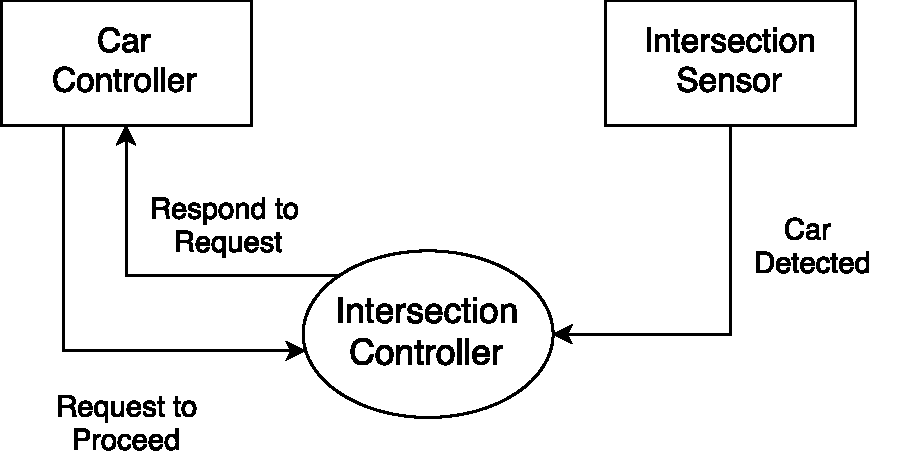
\includegraphics [scale = 0.8] {figures/IC_ContextDiagram.pdf}
	\caption{Intersection Controller Context Diagram}
\end{figure}
\break
\begin{figure} [h!]
	\centering
	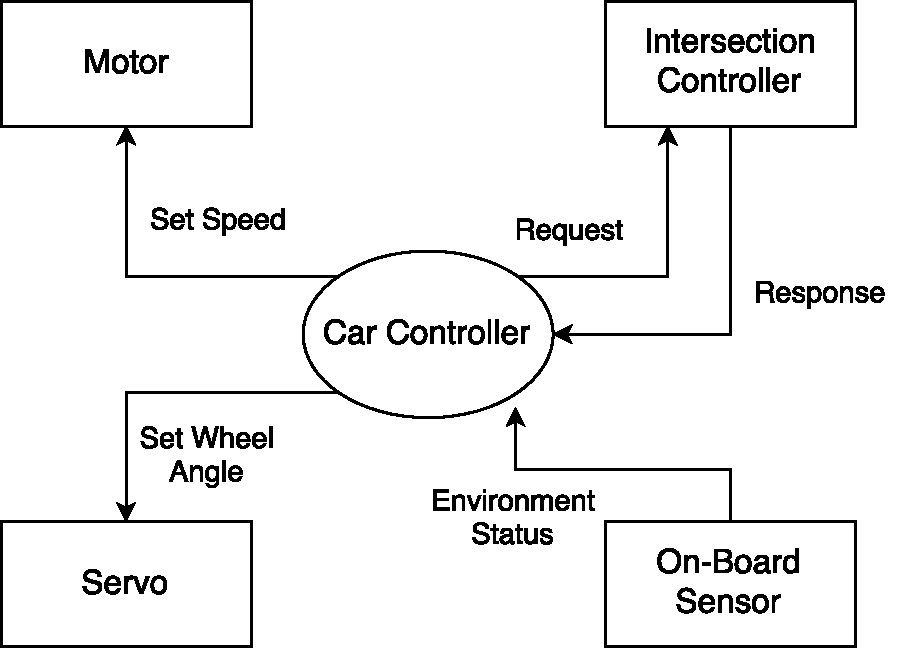
\includegraphics [scale =0.8] {figures/CarCtrl_ContextDiag.pdf}
	\caption{Car Controller Context Diagram}
\end{figure}








%---------------------------- Functional Requirements ------------------------%

\section {Functional Requirements} 
The requirements for this project are separated into the three main components of the system: the track, vehicle, and intersection controller.



% Track Requirements

% if one requirements gets deleted it will be shown in the requirement likelihood of change as ??
% with all the other labels numbers updated

 % ------ NOTE ------% 
% CAN ONLY ADD REQUIREMENTS TO END OF LIST WITH OWN UNIQUE LABEL
% Which would then have to be put at the end of the requirement group in likelihood of change section
% If we add requirements in the middle, the likelihood of change will get messed up

\subsection{Track Functional Requirements}

\begin{longtable}{| p{.2\textwidth } | p{.75\textwidth } | }\hline 
\rowcolor{tableCell}\textbf{T1} & The track must have 30 $\pm 1$ cm wide lanes \\ \hline
\textbf{Rationale} & In order to fit $\frac{1}{10}$ scale vehicles \\ \hline 

\end{longtable}

\begin{longtable}{| p{.2\textwidth } | p{.75\textwidth } | }\hline 
\rowcolor{tableCell}\textbf{T2} & The track must have an intersection \\ \hline
\textbf{Rationale} &  Provide a testable environment\\ \hline 

\end{longtable}

\begin{longtable}{| p{.2\textwidth } | p{.75\textwidth } | }\hline 
\rowcolor{tableCell}\textbf{T3} &  The track must have objects to indicate stopping at the intersection\\ \hline
\textbf{Rationale} & To allow the vehicle to identify the intersection \\ \hline 
\end{longtable}

\begin{longtable}{| p{.2\textwidth } | p{.75\textwidth } | }\hline 
\rowcolor{tableCell}\textbf{T4} & The track must have objects to indicate the direction \\ \hline
\textbf{Rationale} &  To allow the vehicle to identify direction it is coming from and going to\\ \hline 


\end{longtable}



% Vehicle Requirements
\subsection{Vehicle Functional Requirements}


\begin{longtable}{| p{.2\textwidth } | p{.75\textwidth } | }\hline 
\rowcolor{tableCell}\textbf{V1} & The vehicle must be able to send and receive signals to and from the intersection controller \\ \hline
\textbf{Rationale} &  Provide a means for the vehicles to pass and receive information to and from the intersection controller\\ \hline 
\end{longtable}

\begin{longtable}{| p{.2\textwidth } | p{.75\textwidth } | }\hline 
\rowcolor{tableCell}\textbf{V2} & The vehicle must be able to detect lanes and follow them \\ \hline
\textbf{Rationale} &  To follow an intended path\\ \hline 

\end{longtable}

\begin{longtable}{| p{.2\textwidth } | p{.75\textwidth } | }\hline 
\rowcolor{tableCell}\textbf{V3} & The vehicle must be able to detect intersections \\ \hline
\textbf{Rationale} &  To be able know where to stop at the intersection\\ \hline 

\end{longtable}

\begin{longtable}{| p{.2\textwidth } | p{.75\textwidth } | }\hline 
\rowcolor{tableCell}\textbf{V4} & The vehicle must be able to stop at intersections \\ \hline
\textbf{Rationale} & To avoid collisions and follow rules of the road \\ \hline 

\end{longtable}

\begin{longtable}{| p{.2\textwidth } | p{.75\textwidth } | }\hline 
\rowcolor{tableCell}\textbf{V5} & The vehicle must be able to navigate through intersections \\ \hline
\textbf{Rationale} & To continue following the intended path after arriving at the intersection \\ \hline 

\end{longtable}

\begin{longtable}{| p{.2\textwidth } | p{.75\textwidth } | }\hline 
\rowcolor{tableCell}\textbf{V6} & The vehicle must be able to avoid obstacles \\ \hline
\textbf{Rationale} &  To prevent collisions and damage to vehicle and surrounding property\\ \hline 

\end{longtable}






% VI Controller Requirements

\subsection{Intersection Controller Functional Requirements}
\begin{longtable}{| p{.2\textwidth } | p{.75\textwidth } | }\hline 
\rowcolor{tableCell}\textbf{IC1} & The intersection controller must be able to detect if there is a car at the intersection  \\ \hline
\textbf{Rationale} &  To make safe and informed decisions \\ \hline 
\end{longtable}

\begin{longtable}{| p{.2\textwidth } | p{.75\textwidth } | }\hline 
\rowcolor{tableCell}\textbf{IC2} & The intersection controller must be able to detect when a car has exited the intersection \\ \hline
\textbf{Rationale} &  Confirmation vehicles has left the intersection to allow safe and informed decision \\ \hline 
\end{longtable}

\begin{longtable}{| p{.2\textwidth } | p{.75\textwidth } | }\hline 
\rowcolor{tableCell}\textbf{IC3} & The intersection controller must be able to determine the order in which the cars should proceed \\ \hline
\textbf{Rationale} & To ensure a fair and safe scheduling policy \\ \hline 
\end{longtable}

\begin{longtable}{| p{.2\textwidth } | p{.75\textwidth } | }\hline 
\rowcolor{tableCell}\textbf{IC4} & The intersection controller must be able to receive signals from the vehicles  \\ \hline
\textbf{Rationale} &  Alter the intersection when the vehicle wishes to proceed through the intersection\\ \hline 
\end{longtable}

\begin{longtable}{| p{.2\textwidth } | p{.75\textwidth } | }\hline 
\rowcolor{tableCell}\textbf{IC5} & The intersection controller must be able to signal to the vehicle when it is allowed to go through the intersection \\ \hline
\textbf{Rationale} &  Alert the vehicle when it should proceed\\ \hline 
\end{longtable}

\begin{longtable}{| p{.2\textwidth } | p{.75\textwidth } | }\hline 
\rowcolor{tableCell}\textbf{IC6} & The system must have two modes of operation, namely: traffic optimization and traditional traffic rules \\ \hline
\textbf{Rationale} & Fulfill projects constraints outlined by the client \\ \hline 
\end{longtable}



\section{Functional Decomposition Diagrams}
\begin{figure} [h!]
	\caption{Functional Intersection Controller Decomposition}\bigskip
	\centering
	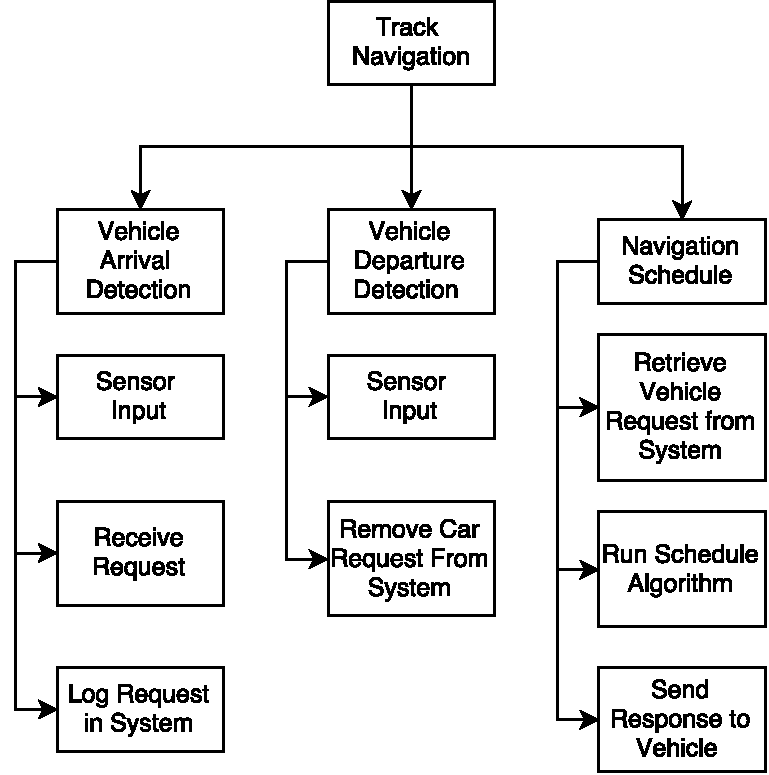
\includegraphics [scale =.8] {figures/function_decomp_IC.pdf}
	
\end{figure}

\pagebreak

\begin{figure} [h!]
	\caption{Functional Track Navigation Decomposition}\bigskip
	\centering
	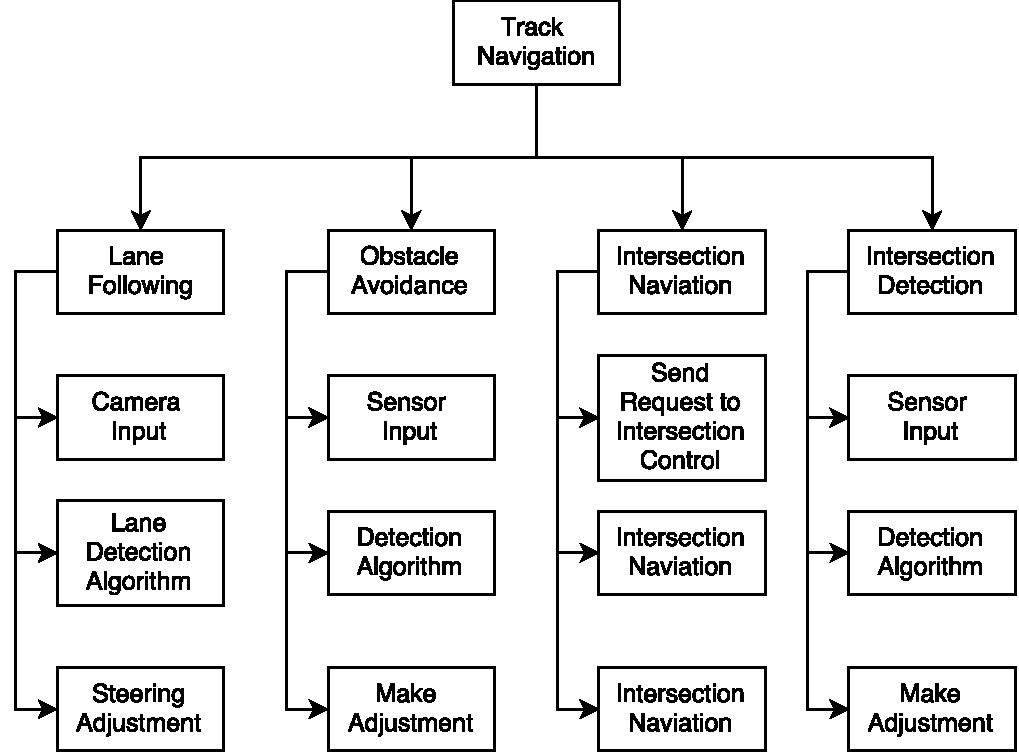
\includegraphics [scale =.8] {figures/function_decomp_track_n.pdf}
	
\end{figure}





\section{Functional Requirements Likelihood of Change} 

\subsection{Track}
\begin{longtable}{| p{.15\textwidth } | p{.14\textwidth } |  p{.3\textwidth } | p{.30\textwidth } |}\hline 
\multicolumn{1}{|c|}{\textbf {Requirement}} & 
\begin{minipage}{.14 \columnwidth}\begin{center}\vspace{1.5mm}\textbf{Change Likelihood}   \vspace{1.5mm} \end{center}\end{minipage}& 
\multicolumn{1}{c|}{\textbf {Rationale}} & \multicolumn{1}{c|}{\textbf {Ways to Change}} \\ \hline

\rowcolor{tableCell} \multicolumn{1}{|c|}{T1}& 
\multicolumn{1}{|c|}{Very Unlikely} & Mandated constraint & N/A \\ \hline
\multicolumn{1}{|c|}{T2}& 
\multicolumn{1}{|c|}{Very Unlikely} & Mandated constraint & N/A  \\ \hline
\rowcolor{tableCell} \multicolumn{1}{|c|}{T3}& 
\multicolumn{1}{|c|}{Very Unlikely} & Mandated constraint & N/A  \\ \hline

\multicolumn{1}{|c|}{T4}& 
\multicolumn{1}{|c|}{Likely} & Subject to consent of other groups& Means of direction identification could change  \\ \hline

\end{longtable}

\subsection{Vehicle}
\begin{longtable}{| p{.15\textwidth } | p{.14\textwidth } |  p{.3\textwidth } | p{.30\textwidth } |}\hline 
\multicolumn{1}{|c|}{\textbf {Requirement}} & 
\begin{minipage}{.14 \columnwidth}\begin{center}\vspace{1.5mm}\textbf{Change Likelihood}   \vspace{1.5mm} \end{center}\end{minipage}& 
\multicolumn{1}{c|}{\textbf {Rationale}} & \multicolumn{1}{c|}{\textbf {Ways to Change}} \\ \hline

 \rowcolor{tableCell}\multicolumn{1}{|c|}{V1}& \multicolumn{1}{|c|}{Very Unlikely}& Key implementation aspect & N/A  \\ \hline
 \multicolumn{1}{|c|}{V2}& \multicolumn{1}{|c|}{Very Unlikely}& Key implementation aspect & N/A  \\ \hline
\rowcolor{tableCell} \multicolumn{1}{|c|}{V3}& \multicolumn{1}{|c|}{Very Unlikely}& Key implementation aspect & N/A  \\ \hline
 \multicolumn{1}{|c|}{V4}& \multicolumn{1}{|c|}{Very Unlikely}& Key implementation aspect & N/A  \\ \hline
\rowcolor{tableCell} \multicolumn{1}{|c|}{V5}& \multicolumn{1}{|c|}{Very Unlikely}& Key implementation aspect & N/A  \\ \hline
 \multicolumn{1}{|c|}{V6}& \multicolumn{1}{|c|}{Likely}& This requirement has a lower priority compared to other requirements, and it is subject to time constraints & Requirement may be removed \\ \hline
\end{longtable}

\subsection{Intersection Controller}

\begin{longtable}{| p{.15\textwidth } | p{.14\textwidth } |  p{.3\textwidth } | p{.30\textwidth } |}\hline 
\multicolumn{1}{|c|}{\textbf {Requirement}} & 
\begin{minipage}{.14 \columnwidth}\begin{center}\vspace{1.5mm}\textbf{Change Likelihood}   \vspace{1.5mm} \end{center}\end{minipage}& 
\multicolumn{1}{c|}{\textbf {Rationale}} & \multicolumn{1}{c|}{\textbf {Ways to Change}} \\ \hline

\rowcolor{tableCell} \multicolumn{1}{|c|}{IC1}& \multicolumn{1}{|c|}{Very Unlikely}& Key implementation aspect & N/A \\ \hline
\multicolumn{1}{|c|}{IC2}&\multicolumn{1}{|c|}{Likely} & IC may not be able to accurately detect when the vehicle has left the intersection & System can be configured such that the vehicle directly informs the IC when it has left the intersection \\ \hline
\rowcolor{tableCell} \multicolumn{1}{|c|}{IC3}&\multicolumn{1}{|c|}{Very Unlikely} & Key implementation aspect & N/A \\ \hline
\multicolumn{1}{|c|}{IC4}&\multicolumn{1}{|c|}{Very Unlikely} & Key implementation aspect & N/A \\ \hline
\rowcolor{tableCell} \multicolumn{1}{|c|}{IC5}&\multicolumn{1}{|c|}{Very Unlikely} & Key implementation aspect & N/A \\ \hline
\multicolumn{1}{|c|}{IC6}&\multicolumn{1}{|c|}{Likely} & This requirement has a lower priority compared to other requirements, and it is subject to time constraints & Requirement may be removed \\ \hline


\end{longtable}




%---------------------------- Nonfunctional Requirements ------------------------%

\section {Nonfunctional Requirements} 



\subsection {Look and Feel Requirements}
\subsubsection{Appearance Requirements}
	\begin{itemize}
		\item  N/A
	\end{itemize}
	% This is a test section


\subsubsection{Style Requirements}
	\begin{itemize}
		\item N/A
	\end{itemize}

\subsection{Usability and Humanity Requirements} 
\subsubsection{Ease of Use Requirements}
	\begin{itemize}
		\item N/A
	\end{itemize}

\subsubsection{Personalization and Internationalization Requirements}
	\begin{enumerate}[label=\textbf{\Alph*}:]
		\item The vehicle must drive on the right side of the lanes
	\end{enumerate}

\subsubsection{Learning Requirements }
	\begin{itemize}
		\item N/A
	\end{itemize}

\subsubsection{Understandability and Politeness Requirements}
	\begin{itemize}
		\item N/A
	\end{itemize}
		
\subsubsection{Accessibility Requirements }
	\begin{itemize}
		\item N/A
	\end{itemize}
 
\subsection{Performance Requirements}

\subsubsection{Speed Requirements }
	\begin{enumerate}[label=\textbf{\Alph*}:]
		\item The system must be able to determine an order and convey it to the vehicle before a soft deadline
		\item The system must capture and process intersection information within 0.3 seconds
		\item The vehicle must process the state of the track in less than 0.3 seconds
	\end{enumerate}

\subsubsection{Safety-Critical Requirements }
	\begin{enumerate}[label=\textbf{\Alph*}:]
		\item The system must only signal a car to proceed when the intersection is clear
		\item The vehicle must stop within a safe distance of an obstacle
		\item The system must have an emergency shutdown mode
	\end{enumerate}	


\subsubsection{Precision Requirements}
	\begin{enumerate}[label=\textbf{\Alph*}:]
		\item The vehicle must not deviate from the lanes more than 10\%
	\end{enumerate}

\subsubsection{Reliability or Availability  Requirements}
	\begin{enumerate}[label=\textbf{\Alph*}:]
		\item The system must operate without failure 95\% of the time
		\item The vehicle system must operate as long as the car's internal power supply is charged
	\end{enumerate}



\subsubsection{Robustness or Fault-Tolerance Requirements }
	\begin{enumerate}[label=\textbf{\Alph*}:]
		\item In the event of a complete vehicle system failure, the vehicle must come to a stop within 10cm
	\end{enumerate}
	
\subsubsection{Capacity Requirements }
	\begin{enumerate}[label=\textbf{\Alph*}:]
		\item The intersection controller must be able to manage at least one intersection at a time
		\item The intersection controller shall be able to communicate with a maximum of four cars at a time
	\end{enumerate}

\subsubsection{Scalability or Extensibility Requirements }
	\begin{itemize}
		\item N/A
	\end{itemize}
		
\subsubsection{Longevity Requirements }
	\begin{enumerate}[label=\textbf{\Alph*}:]
		\item Components should be functional for up to one year
	\end{enumerate}

% Operational and Environmental Requirements
\subsection{Operational and Environmental Requirements}
\subsubsection{Expected Physical Environment }
	\begin{enumerate}[label=\textbf{\Alph*}:]
		\item The track must be 1/10 scale of a real world intersection
		\item The vehicle must be able to operate on a track in a lab setting
	\end{enumerate}
		
\subsubsection{Requirements for Interacting with Adjacent Systems}
	\begin{enumerate}[label=\textbf{\Alph*}:]
		\item The components must be able to use the API of existing and partner components
	\end{enumerate}

\subsection{Maintainability and Support Requirements }
\subsubsection{Maintenance Requirements }
	\begin{enumerate}[label=\textbf{\Alph*}:]
		\item  Issues must be resolved within one week of discovering an error in the system
	\end{enumerate}

\subsubsection{Supportability Requirements }
	\begin{itemize}
		\item N/A
	\end{itemize}

\subsubsection{Adaptability Requirements}
	\begin{itemize}
		\item N/A
	\end{itemize}

\subsection{Security Requirements }
\subsubsection{Access Requirements }
	\begin{enumerate}[label=\textbf{\Alph*}:]
		\item All stated stakeholders have full access to the product
	\end{enumerate}

\subsubsection{Integrity Requirements }
	\begin{enumerate}[label=\textbf{\Alph*}:]
		\item The system will not be altered by external malicious Bluetooth signals
	\end{enumerate}

\subsubsection{Privacy Requirements }
	\begin{enumerate}[label=\textbf{\Alph*}:]
		\item Image data gathered by the vehicle controller will not be stored 
		\item Image data gathered by the intersection controller will not be stored
		\item Information passed between the vehicle and the intersection must not include sensitive information
		\item All message passing between subsystem will be encrypted
	\end{enumerate}

\subsubsection{Audit  Requirements }
	\begin{itemize}
		\item N/A
	\end{itemize} 

\subsubsection{Immunity Requirements  }
	\begin{itemize}
		\item N/A
	\end{itemize}

\subsection{Cultural and Political Requirements } 
\subsubsection{Cultural Requirements }
	\begin{itemize}
		\item N/A
	\end{itemize}

\subsubsection{Political Requirements }
	\begin{itemize}
		\item N/A
	\end{itemize}


\subsection{Legal Requirements}
\subsubsection{Compliance Requirements }
	\begin{itemize}
		\item N/A
	\end{itemize}
	
\subsubsection{Standards Requirements }
	\begin{itemize}
		\item N/A
	\end{itemize}


%---------------------------- Project Issues ------------------------%

\section {Project Issues} 


\subsection{Open Issues}
	\begin{itemize}
		\item  None
	\end{itemize}

\subsection{Off-the-Shelf Solutions}

\subsubsection{Ready-Made Products}
	\begin{enumerate}[label=\textbf{\Alph*}:]
		\item OpenCV  - existing software used for image processing
		\item BlueZ - a Bluetooth library
	\end{enumerate}


\subsection{Risks}
	\begin{enumerate}[label=\textbf{\Alph*}:]
		\item Component failure - Failure of components can result in damage to the remote control cars.
		\item Damaged parts - Damaged parts will result in delay of the project and will require more parts to be bought.
		\item Potential of minor injuries to humans - Humans can be injured if parts malfunction. 
	\end{enumerate}
	

	
\subsection{Costs}	
		
		The general budget for the major components are as follow:

		\begin{enumerate}[label=\textbf{\Alph*}:]
			\item 1/10th model car (x2) \$240.00 each
			\item Cameras and sensors \$50.00
			\item Vehicle Battery (x2) and Charger \$90.00
			\item Raspberry Pi (x2) \$150.00
		\end{enumerate}
		
		Total Cost : \$530.00


\subsection{Waiting Room}
	\begin{enumerate}[label=\textbf{\Alph*}:]
		\item Having the system work with other autonomous car models
	    \end{enumerate} 



\end{document}
